\documentclass[tikz,border=5pt]{standalone}
\usepackage[UTF8]{ctex}
\usepackage{amsmath,amssymb}
\usetikzlibrary{arrows.meta,calc,angles,quotes,patterns,decorations.pathmorphing}
\definecolor{field}{HTML}{176B9B}
\definecolor{force}{HTML}{B64B32}
\tikzset{>=Latex,line width=.8pt,every node/.style={font=\small},field/.style={color=field},force/.style={color=force},body/.style={draw=black,fill=blue!6},ghost/.style={dashed,gray},labelbox/.style={fill=white,inner sep=1.5pt}}
\begin{document}
\begin{tikzpicture}
% Spatial projection of the paraboloid, with rear rim hidden.
\draw[body] (-1.6,2.5) .. controls (-1.25,1.15) and (-.7,.25) .. (0,0)
 .. controls (.7,.25) and (1.25,1.15) .. (1.6,2.5);
\draw[ghost] (1.6,2.5) arc (0:180:1.6 and .42);
\draw (-1.6,2.5) arc (180:360:1.6 and .42);
\draw[ghost] (0,0) .. controls (-.4,.8) and (-.45,1.8) .. (0,2.08);
\draw (0,0) .. controls (.4,.8) and (.45,1.8) .. (0,2.92);
\draw[dash dot] (0,0)--(0,3.4) node[above] {对称轴};
\fill (0,.85) circle (1.8pt) node[right=4pt] {$C$};
\draw[<->] (-.55,0)--(-.55,.85) node[midway,left] {$h$};
\draw[thick] (-2.1,-.03)--(2.1,-.03);
\node[below] at (0,-.03) {水平支持面};
\node[right] at (2,1.5) {旋转抛物面};
\end{tikzpicture}
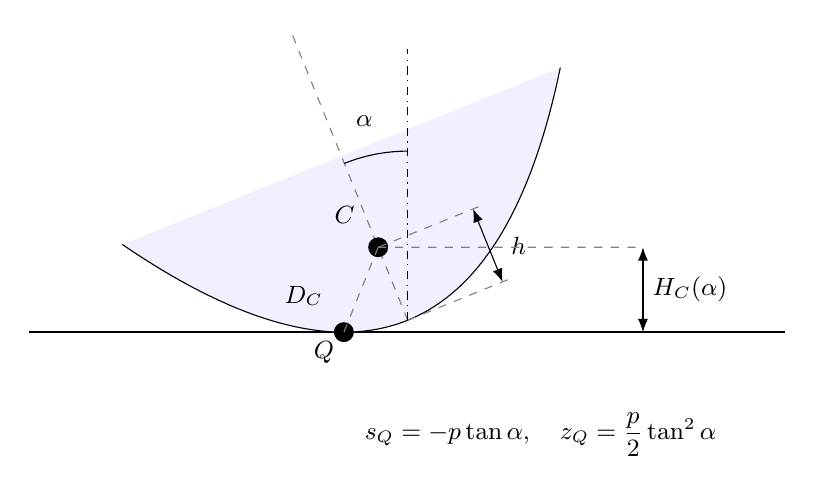
\begin{tikzpicture}[scale=2]
\def\a{22}
\draw[thick] (-2,0)--(2.8,0);
\begin{scope}[shift={(.406,.076)},rotate=22]
\draw[body,domain=-1.5:1.5,samples=70] plot (\x,{.5*\x*\x});
\draw[ghost] (0,0)--(0,2.0);
\coordinate(C) at (0,.5);
\coordinate(Q) at (-.404,.0817);
\fill(C) circle(1.8pt) node[above left=5pt] {$C$};
\draw[<->] (.65,0)--(.65,.5) node[midway,right=5pt] {$h$};
\draw[ghost](0,0)--(.7,0);\draw[ghost](0,.5)--(.7,.5);
\end{scope}
\fill(Q)circle(1.8pt) node[below left] {$Q$};
\draw[ghost] (C)--(Q);\node[left] at(-.07,.23) {$D_C$};

\draw[dash dot] (.406,.076)--(.406,1.8);
\draw (.406,1.15) arc(90:112:1.074);
\node at (.13,1.34) {$\alpha$};
\draw[<->] (1.9,0)--(1.9,.5395) node[midway,right] {$H_C(\alpha)$};
\draw[ghost](C)--(1.9,.5395);
\node[below] at (1.25,-.45) {$s_Q=-p\tan\alpha,\quad z_Q=\dfrac p2\tan^2\alpha$};
\end{tikzpicture}
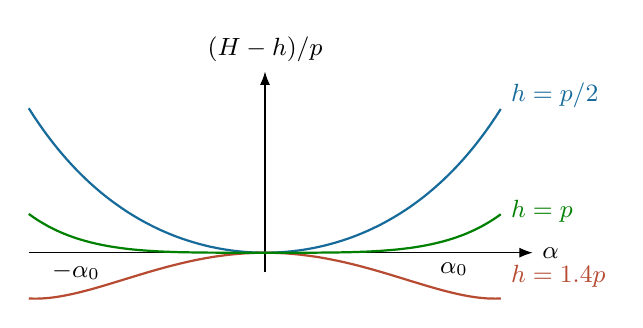
\begin{tikzpicture}
\draw[->] (-3,0)--(3.4,0) node[right] {$\alpha$};
\draw[->] (0,-.25)--(0,2.3) node[above] {$(H-h)/p$};
\draw[field,domain=-.75:.75,samples=100,thick] plot ({4*\x},{10*((.5-.5)*cos(\x r)+.5/cos(\x r)-.5)});
\draw[force,domain=-.75:.75,samples=100,thick] plot ({4*\x},{10*((1.4-.5)*cos(\x r)+.5/cos(\x r)-1.4)});
\draw[green!50!black,domain=-.75:.75,samples=100,thick] plot ({4*\x},{10*((1-.5)*cos(\x r)+.5/cos(\x r)-1)});
\node[field,right] at (3,2.0) {$h=p/2$};
\node[green!50!black,right] at (3,.52) {$h=p$};
\node[force,right] at (3,-.3) {$h=1.4p$};
\node[below] at (-2.4,0) {$-\alpha_0$};
\node[below] at (2.4,0) {$\alpha_0$};
\end{tikzpicture}
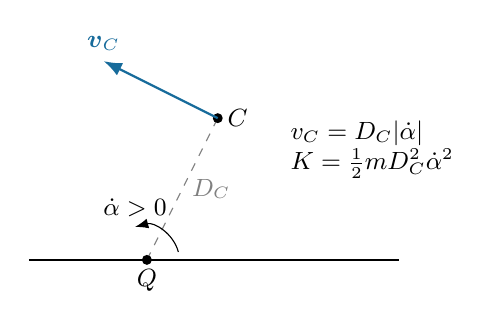
\begin{tikzpicture}
\draw[thick] (-1.5,0)--(3.2,0);
\coordinate(Q) at(0,0);\coordinate(C) at(.9,1.8);
\draw[ghost] (Q)--(C) node[midway,right] {$D_C$};
\fill(Q)circle(1.8pt)node[below]{$Q$};
\fill(C)circle(1.8pt)node[right]{$C$};
\draw[->,field,thick] (C)--(-.55,2.525) node[above] {$\boldsymbol v_C$};
\draw[->] (.4,.1) arc(15:105:.45) node[above] {$\dot\alpha>0$};
\node[right,align=left] at (1.7,1.4) {$v_C=D_C|\dot\alpha|$\\$K=\tfrac12mD_C^2\dot\alpha^2$};
\end{tikzpicture}
\end{document}
